\documentclass{standalone}
\usepackage{tikz}
\usetikzlibrary{arrows.meta, decorations.pathreplacing}
\begin{document}

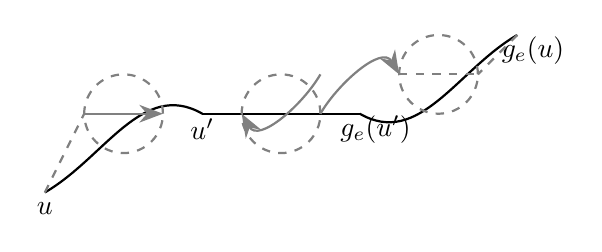
\begin{tikzpicture}[scale=1]

% Draw main curves
\draw[thick] (-3,-1) to[out=30,in=150] (-1,0); % Left curve
\draw[thick] (-1,0) -- (1,0); % Straight line segment
\draw[thick] (1,0) to[out=-30,in=-150] (3,1); % Right curve

% Draw dashed circles
\draw[dashed, gray, thick] (-2,0) circle (0.5); % Circle around u'
\draw[dashed, gray, thick] (0,0) circle (0.5); % Circle around middle point
\draw[dashed, gray, thick] (2,0.5) circle (0.5); % Circle around g_e(u')

% Place nodes for labels
\node at (-3,-1.2) {$u$}; % Label for u
\node at (-1,-0.2) {$u'$}; % Label for u'
\node at (1.2,-0.2) {$g_e(u')$}; % Label for g_e(u')
\node at (3.2,0.8) {$g_e(u)$}; % Label for g_e(u)

% Draw curved arrows
\draw[-{Stealth[length=3mm]}, gray, thick] (0.5,0) to[out=60,in=120] (1.5,0.5); % Arrow from middle to g_e(u')
\draw[-{Stealth[length=3mm]}, gray, thick] (-2.5,0) -- (-1.5,0); % Arrow from left side to u'
\draw[-{Stealth[length=3mm]}, gray, thick] (0.5,0.5) to[out=240,in=300] (-0.5,0); % Arrow from right side to middle

% Additional diagonal lines
\draw[dashed, gray, thick] (-3,-1) -- (-2.5,0); % Diagonal line near u
\draw[dashed, gray, thick] (-2.5,0) -- (-1.5,0); % Diagonal line near u'
\draw[dashed, gray, thick] (3,1) -- (2.5,0.5); % Diagonal line near g_e(u)
\draw[dashed, gray, thick] (1.5,0.5) -- (2.5,0.5); % Diagonal line near g_e(u')

\end{tikzpicture}

\end{document}